% JACoW-style working scaffold for the Hessian-SVD correction paper.
% Scientific claims are intentionally limited to the transferred parity study.
\documentclass[letterpaper]{jacow}

\usepackage[english]{babel}
\usepackage{bm}

\begin{document}

\title{HESSIAN-SVD NONLINEAR CLOSED-ORBIT CORRECTION IN A CESR MODEL BASED ON SciBMAD}

% TODO: Replace the temporary author metadata before circulation/submission.
\author[1]{J. N. Author\thanks{TODO: corresponding-author email}}
\affil[1]{Cornell University, Ithaca, NY, USA}

\maketitle

\begin{abstract}
\textbf{Placeholder.} The completed abstract will state the closed-orbit
correction problem, the Hessian-SVD method, the correction experiments, and
the demonstrated validity boundary.  No correction result is claimed in this
working scaffold.
\end{abstract}

\section{Introduction}

\textbf{Placeholder.} This section will motivate finite-amplitude closed-orbit
correction, connect the problem to the previously established nonlinear
response-error analysis, and define the contribution of the Hessian-SVD
approach.  The literature context and final paper outline remain to be added.

\section{Problem Definition and Notation}

\textbf{Placeholder.} This section will define the detector orbit, corrector
vector, linear response matrix, Hessian tensor, objective function, constraints,
and normalization used by the correction study.  It will also specify the CESR
model and the exact nonlinear reference calculation shared by all comparisons.

\section{Hessian-SVD Formulation}

\textbf{Placeholder.} This section will derive the projected Hessian
representation and its singular-value decomposition, including truncation,
regularization, and the relationship to conventional linear-SVD orbit
correction.  Algorithmic details will be added only after the formulation has
been implemented and verified.

\section{Correction Algorithm and Experiments}

\textbf{Placeholder.} This section will define the correction workflow,
baselines, evaluation states, convergence criteria, and performance metrics.
Tables and figures will be inserted after the correction experiments are
complete; no numerical correction performance is asserted here.

\section{Higher-Order Validity Boundary}

The Hessian correction model is quadratic in the corrector increment.  Its
useful operating range is therefore channel dependent whenever the first
neglected odd contribution becomes comparable with the retained even
contribution.  An existing vertical-only signed-parity experiment provides a
concrete model-order boundary that will be reused when selecting correction
step sizes and deciding when exact nonlinear re-evaluation is required.

Let $\bm r(\Delta\bm k)$ denote the nonlinear orbit residual after subtracting
the nominal linear prediction $J\Delta\bm k$.  Paired positive and negative
inputs separate its even and odd parts,
\begin{equation}
  \begin{aligned}
    \bm r_{\mathrm{even}}(\Delta\bm k)
    &=\frac{\bm r(+\Delta\bm k)+\bm r(-\Delta\bm k)}{2},\\
    \bm r_{\mathrm{odd}}(\Delta\bm k)
    &=\frac{\bm r(+\Delta\bm k)-\bm r(-\Delta\bm k)}{2}.
  \end{aligned}
  \label{eq:parity-decomposition}
\end{equation}
The experiment used 100 fixed vertical-corrector directions at 27 input radii,
for 5401 states including the nominal state.  All states converged without
fallback.  In the vertical detector channel, the even residual followed the
expected quadratic trend and the odd nonlinear residual followed a cubic
trend.  Their fitted mean rms trends crossed at $\rho=1.31$, corresponding to
an active-corrector rms of approximately $6.5\,\mu\mathrm{rad}$.  At
$\rho=6.4$, the mean odd/even ratio was 4.91.  The simultaneous horizontal
control ratio was only $3.05\times10^{-4}$, demonstrating that the breakdown
of a quadratic approximation cannot be assigned from input amplitude alone;
the input and detector channels must also be specified.

\begin{figure}[!htb]
  \centering
  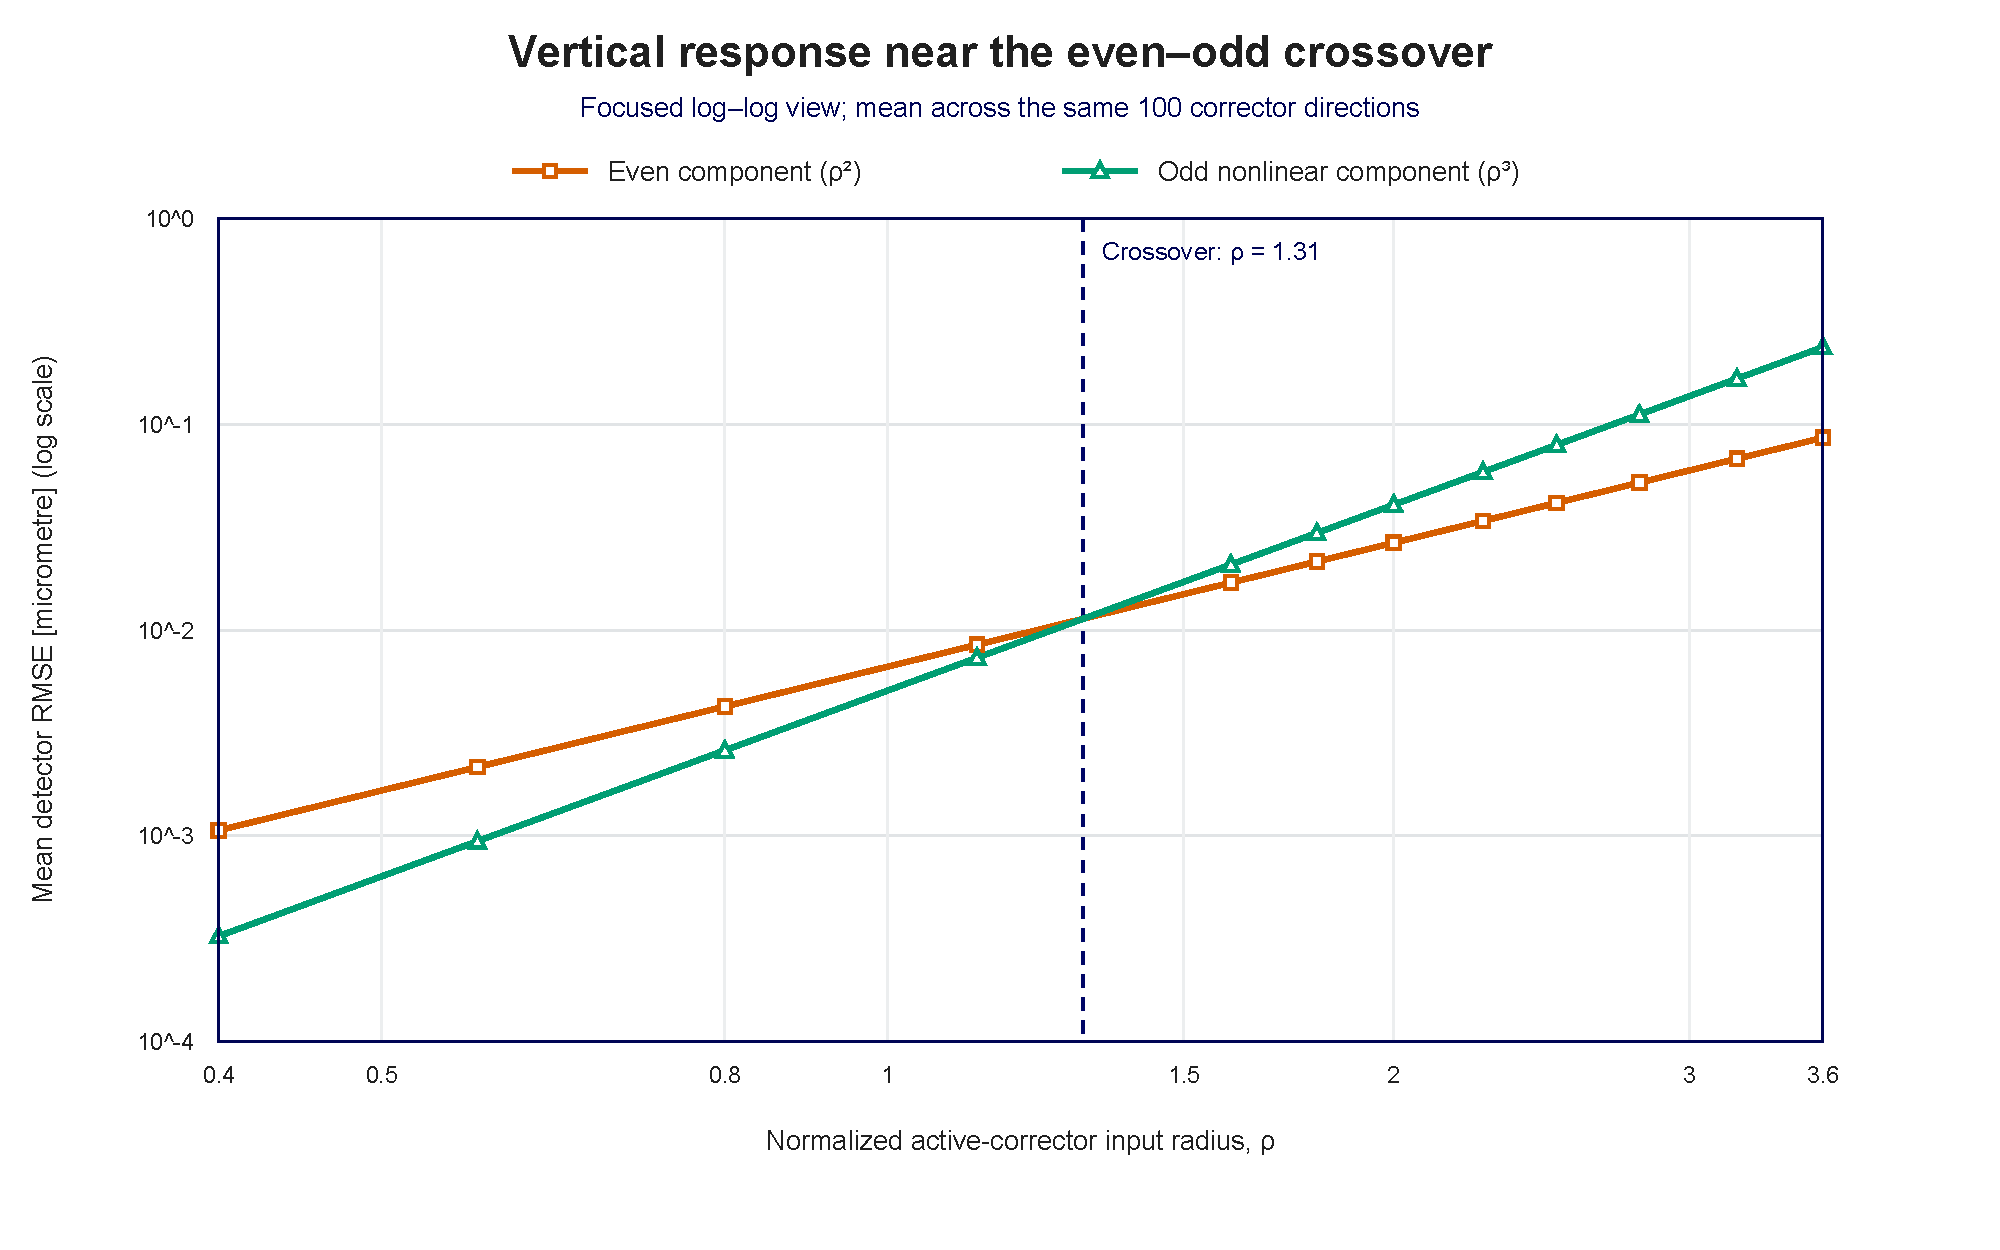
\includegraphics[width=\columnwidth]{figures/vertical_parity_crossover_loglog.pdf}
  \caption{Mean vertical even and odd nonlinear residuals for vertical-only
  inputs.  Their fitted quadratic and cubic trends cross at $\rho=1.31$.}
  \label{fig:vertical-parity-crossover}
\end{figure}

\begin{figure}[!htb]
  \centering
  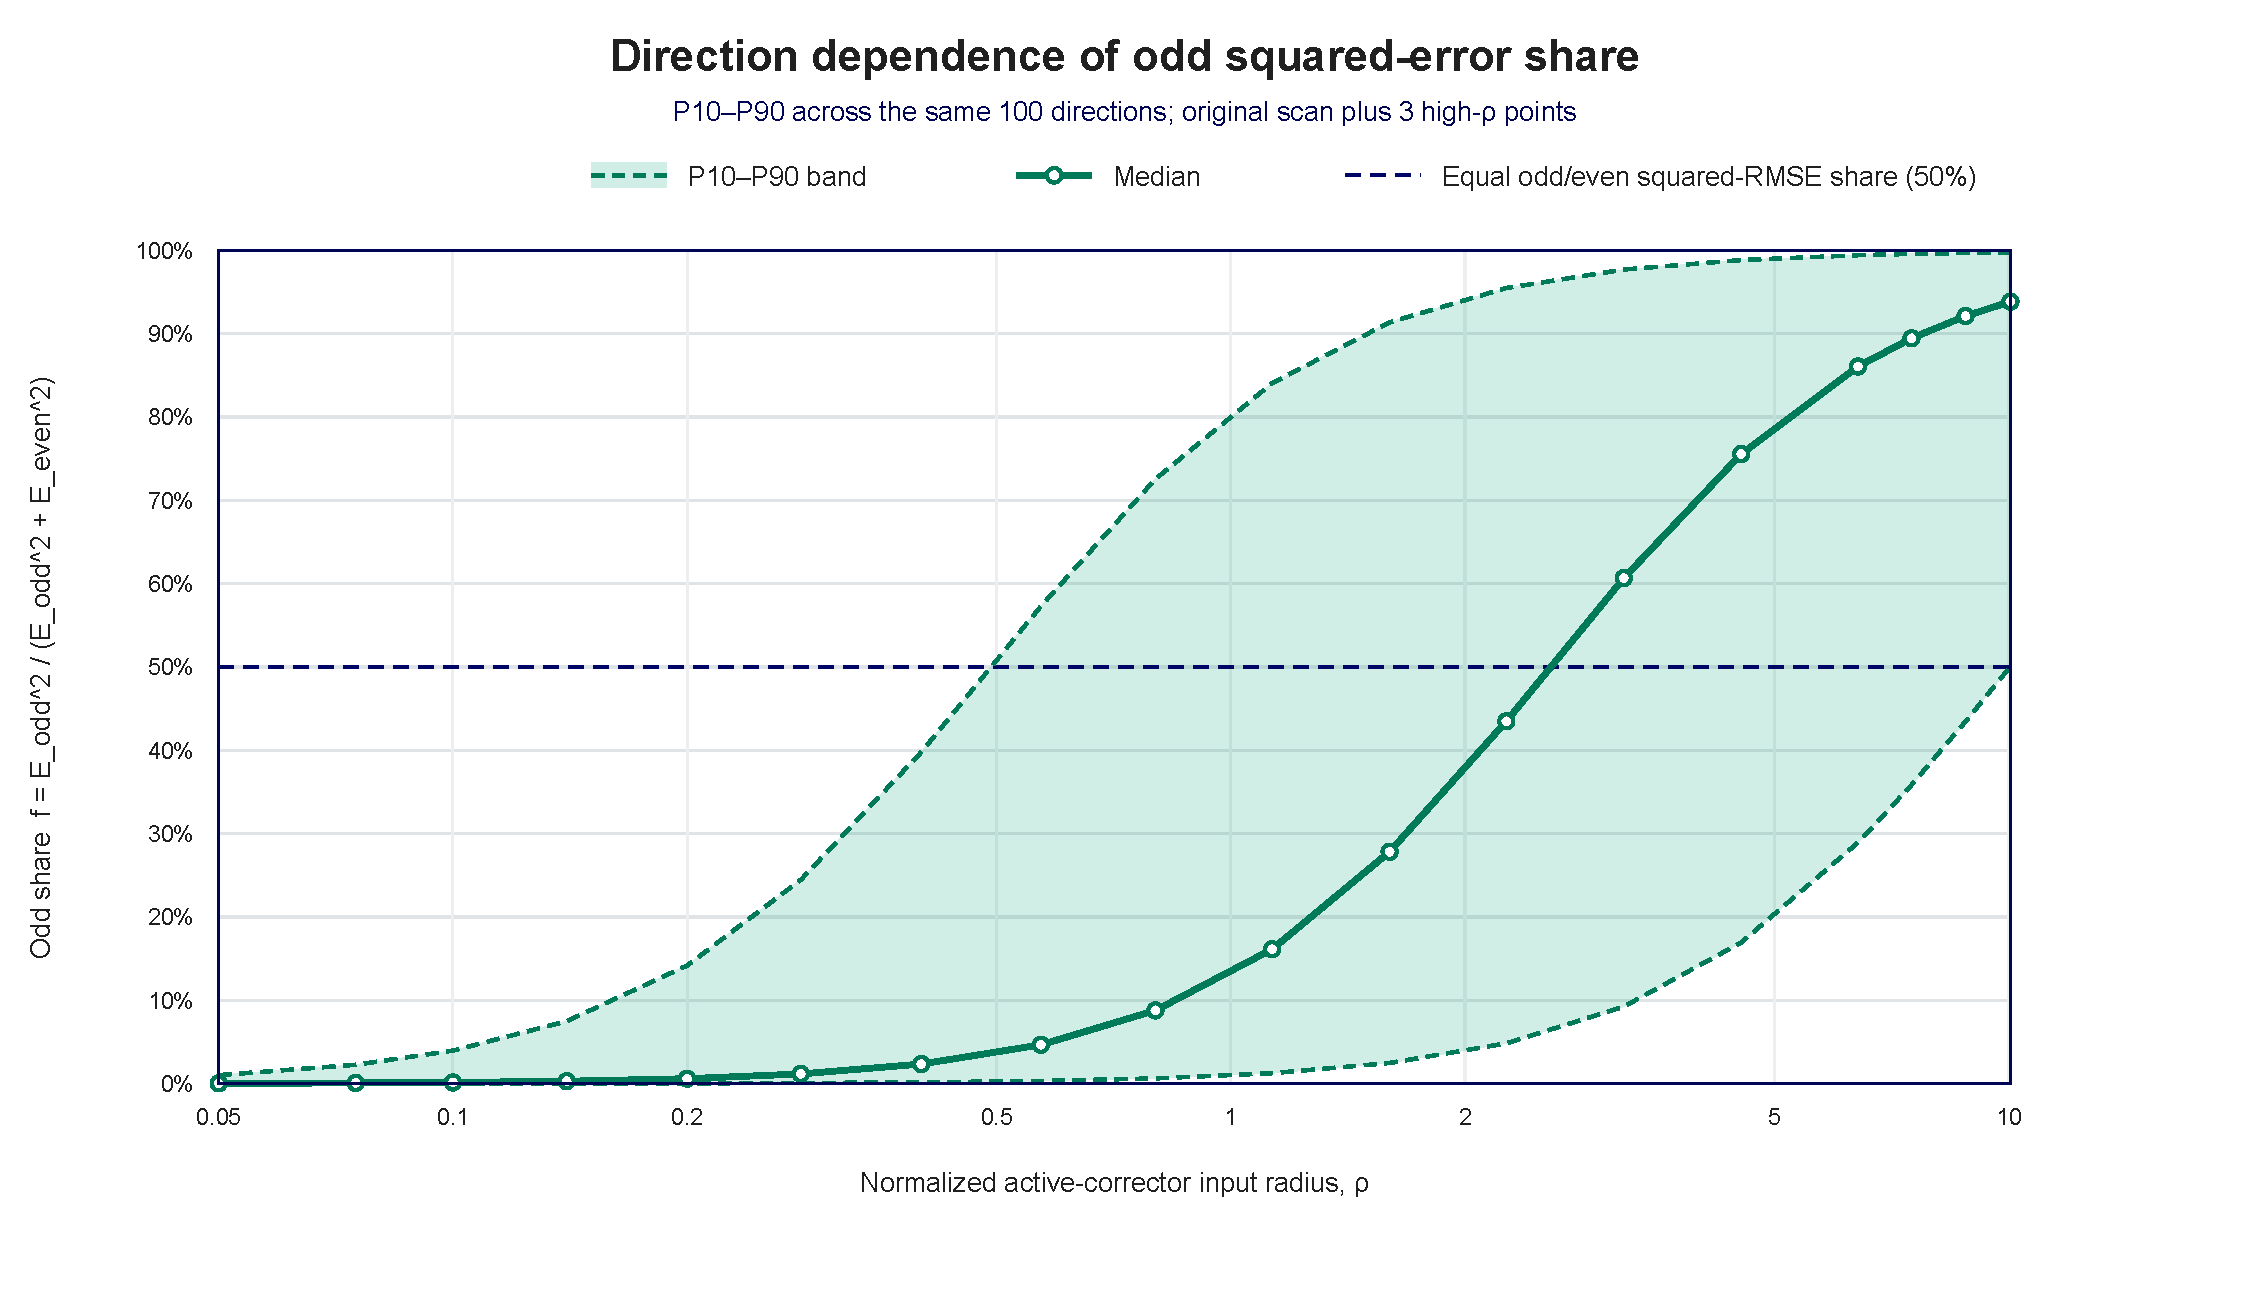
\includegraphics[width=\columnwidth]{figures/vertical_parity_odd_fraction_percentiles.pdf}
  \caption{Odd squared-error share over the same 100 directions.  The line is
  the median and the envelope spans P10--P90, showing strong direction
  dependence despite the small absolute error.}
  \label{fig:vertical-odd-share}
\end{figure}

For the future correction experiments, this result is evidence for a
channel-aware trust region rather than evidence that a particular Hessian-SVD
algorithm succeeds.  The completed study must test whether step restriction,
iteration with exact nonlinear orbit re-evaluation, or a higher-order local
model is required once the vertical odd component becomes significant.  The
physical source of the cubic contribution has not yet been identified.

\section{Conclusion}

\textbf{Placeholder.} The completed conclusion will summarize only verified
correction performance and its model-order limits.  At present, the transferred
parity experiment establishes a candidate validity diagnostic, not a completed
nonlinear orbit-correction result.

\end{document}
